%%%%%%%%%%%%%%%%%%%%%%%%%%%%%%%%%%%%%%%%%%%%%%%
%
% Template for Master degrees
% DISI - Dipartimento di Ingegneria e Scienza dell’Informazione
% DISI - Department of Information Engineering and Computer Science
%
% update 2020-08-30
%
% To generate pdf 
% pdflatex __filename__.tex
% bibtex __file_name__.aux
% pdflatex __file_name__.tex
% pdflatex __file_name__.tex
%
%%%%%%%%%%%%%%%%%%%%%%%%%%%%%%%%%%%%%%%%%%%%%%%

\pdfminorversion=7

% 2 side format
\documentclass[epsfig,a4paper,11pt,titlepage,twoside,openany]{book}
\usepackage{epsfig}
\usepackage{plain}
\usepackage{setspace}
\usepackage[paperheight=29.7cm,paperwidth=21cm,outer=1.5cm,inner=2.5cm,top=2cm,bottom=2cm]{geometry} % layout setting
\usepackage{titlesec} % custom setup title of chapter
\usepackage{url}
\usepackage[]{mdframed} % https://tex.stackexchange.com/a/673010

% Note that you must put this before the \usepackage{hyperref}
% \usepackage[a-1b,mathxmp]{pdfx}[2018/12/22] % PDF/A

% \usepackage{newtxtext,newtxmath} % times new roman

%%%%%%%%%%%%%%
% support for accented letters
%
%\usepackage[latin1]{inputenc} % Windows;
\usepackage[utf8x]{inputenc} % Linux (unicode package is required);
%\usepackage[applemac]{inputenc} % Mac.

\usepackage[pdfa]{hyperref}
\hypersetup{
    colorlinks,
    citecolor=black,
    filecolor=black,
    linkcolor=black,
    urlcolor=black
}
\usepackage[capitalise,noabbrev]{cleveref} % https://ctan.mirror.garr.it/mirrors/ctan/macros/latex/contrib/cleveref/cleveref.pdf

\singlespacing

% italian language
%\usepackage[italian]{babel}

\begin{document}

  % no page number
  \pagenumbering{gobble} 
  \pagestyle{plain}

\thispagestyle{empty}

\begin{center}
  \begin{figure}[h!]
    \centerline{
\psfig{file=marchio_unitrento_colore_it_v2.eps,width=0.6\textwidth}}
  \end{figure}

  \vspace{2 cm} 

  \LARGE{Department of Information Engineering and Computer Science\\}

  \vspace{1 cm} 
  \Large{Master's Degree in\\
    % ...
    Computer Science
    % Computer, Communication and Electronic Engineering
    % Information and Communications Engineering
    % Information and Business Organization Engineering
    % Electornics and Telecommunications Engineerign
  }

  \vspace{2 cm} 
  \Large\textsc{Final Dissertation\\} 
  \vspace{1 cm} 
  \Huge\textsc{Title\\}
  \Large{\it{Sub-title (optional)}}


  \vspace{2 cm} 
  \begin{tabular*}{\textwidth}{ c @{\extracolsep{\fill}} c }
  \Large{Supervisor} & \Large{Student}\\
  \Large{}& \Large{}\\
  \Large{Arrigo Zanette}& \Large{Federico Cucino}\\
  \Large{Marcello Bellomi (former)}& \Large{}\\
  \end{tabular*}

  \vspace{2 cm} 

  \Large{Academic year 2023/24}
  
\end{center}



  \clearpage
 
%%%%%%%%%%%%%%%%%%%%%%%%%%%%%%%%%%%%%%%%%%%%%%%%%%%%%%%%%%%%%%%%%%%%%%%%%%
%%%%%%%%%%%%%%%%%%%%%%%%%%%%%%%%%%%%%%%%%%%%%%%%%%%%%%%%%%%%%%%%%%%%%%%%%%
%% Note
%%%%%%%%%%%%%%%%%%%%%%%%%%%%%%%%%%%%%%%%%%%%%%%%%%%%%%%%%%%%%%%%%%%%%%%%%%
%% Thanks/Acknowledgements section is optional
%%%%%%%%%%%%%%%%%%%%%%%%%%%%%%%%%%%%%%%%%%%%%%%%%%%%%%%%%%%%%%%%%%%%%%%%%%
%%%%%%%%%%%%%%%%%%%%%%%%%%%%%%%%%%%%%%%%%%%%%%%%%%%%%%%%%%%%%%%%%%%%%%%%%%
  \thispagestyle{empty}

\begin{center}
  {\bf \Huge Acknowledgements}
\end{center}

\vspace{4cm}


\emph{
  First, I would like to thank my academic supervisor, professor Alessandro Marchetto, for the guidance and the support.\\
  I extend my gratitude to Corvina \& Exor International companies for giving me the opportunity to work on this challenging and actual project, in particular to my co-supervisors Marcello and Arrigo for their mentorship, technical assistance and continous feedback during the internship. The hands-on experience and exposure to real-world industrial challenges have been invaluable for both my personal and professional growth.\\
  As always, thanks to my family for their unconditional support, source of strength and motivation.\\
  Last but not least, I would like to say thank you to my friends and all the individuals who have been part of this journey.
}

  \clearpage
  \pagestyle{plain} % no heading, footer with centered page number

  
  % page number with Arabic format
  \mainmatter

%%%%%%%%%%%%%%%%%%%%%%%%%%%%%%%%%%%%%%%%%%%%%%%%%%%%%%%%%%%%%%%%%%%%%%%%%%
%%%%%%%%%%%%%%%%%%%%%%%%%%%%%%%%%%%%%%%%%%%%%%%%%%%%%%%%%%%%%%%%%%%%%%%%%%
%% Note
%%%%%%%%%%%%%%%%%%%%%%%%%%%%%%%%%%%%%%%%%%%%%%%%%%%%%%%%%%%%%%%%%%%%%%%%%%
%% Length: approximately 70 pages.
%% These 70 pages include:
%%   table of contents
%%   abstract
%%   chapters
%% Exclude:
%%   title page
%%   acknowledgments
%%   attachments
%%%%%%%%%%%%%%%%%%%%%%%%%%%%%%%%%%%%%%%%%%%%%%%%%%%%%%%%%%%%%%%%%%%%%%%%%%
%%%%%%%%%%%%%%%%%%%%%%%%%%%%%%%%%%%%%%%%%%%%%%%%%%%%%%%%%%%%%%%%%%%%%%%%%%

    % index
    \tableofcontents
    \clearpage
    
    
    
    % group to define space between chapters
    \begingroup
      % no page break between chapters
      % override clear page commands
      \renewcommand{\cleardoublepage}{} 
      \renewcommand{\clearpage}{} 
      % override format of title chapter
      % from
      %   Chapter X
      %   Title
      % to
      %   X   Title
      
      \titleformat{\chapter}
        {\normalfont\Huge\bfseries}{\thechapter}{1em}{}
        
      \titlespacing*{\chapter}{0pt}{0.59in}{0.02in}
      \titlespacing*{\section}{0pt}{0.20in}{0.02in}
      \titlespacing*{\subsection}{0pt}{0.10in}{0.02in}
      
      % summary / abstract
      \chapter*{Abstract} % no number
\label{abtract}

\addcontentsline{toc}{chapter}{Abstract} % add to index

Lorem ipsum dolor sit amet, consectetur adipiscing elit. Donec sed nunc orci. Aliquam nec nisl vitae sapien pulvinar dictum quis non urna. Suspendisse at dui a erat aliquam vestibulum. Quisque ultrices pellentesque pellentesque. Pellentesque egestas quam sed blandit tempus. Sed congue nec risus posuere euismod. Maecenas ut lacus id mauris sagittis egestas a eu dui. Class aptent taciti sociosqu ad litora torquent per conubia nostra, per inceptos himenaeos. Pellentesque at ultrices tellus. Ut eu purus eget sem iaculis ultricies sed non lorem. Curabitur gravida dui eget ex vestibulum venenatis. Phasellus gravida tellus velit, non eleifend justo lobortis eget.






%%%%%%%%%%%%%%%%%%%%%%%%%%%%%%%%%%%%%%%%%%%%%%%%%%%%%%%%%%%%%%%%%%%%%%%%%%
%%%%%%%%%%%%%%%%%%%%%%%%%%%%%%%%%%%%%%%%%%%%%%%%%%%%%%%%%%%%%%%%%%%%%%%%%%
%% Note
%%%%%%%%%%%%%%%%%%%%%%%%%%%%%%%%%%%%%%%%%%%%%%%%%%%%%%%%%%%%%%%%%%%%%%%%%%
%% The first chapter of the final thesis must contain a summary of a 
%% maximum length of 3 pages, introducing the context and motivations,
%% resuming the problem faced by the student, the techniques used for the
%% investigation and the reached outcomes.
%% If the final thesis is developed in collaboration with other students,
%% the personal contribution of the student has to be underlined.
%%%%%%%%%%%%%%%%%%%%%%%%%%%%%%%%%%%%%%%%%%%%%%%%%%%%%%%%%%%%%%%%%%%%%%%%%%
%%%%%%%%%%%%%%%%%%%%%%%%%%%%%%%%%%%%%%%%%%%%%%%%%%%%%%%%%%%%%%%%%%%%%%%%%%      
      
      %%%%%%%%%%%%%%%%%%%%%%%%%%%%%%%%
      % chapters
      %
      % \input or \include
      %
      \chapter{Introduction}
\label{cha:intro}

Nowadays, cybersecurity is one of the most trending subject of discussion around the world.\\

The \textit{Internet} is growing: the users are growing, therefore the exchanged amount of data are growning, and so the malicious actors are growing, trying to mislead an increasing number of people, regardless they are newbies or experienced ones. Every day hundreds of new vulnerabilities~\cite{cve-details-db} are discovered.

In today's rapidly evolving industrial landscape, the integration of connected devices and smart technologies, commonly referred to as the Internet of Things (IoT), has transformed traditional industries such as manufacturing, energy, and transportation. These connected devices enable real-time monitoring, predictive maintenance, and automation, resulting in enhanced productivity and efficiency. \\
However, the widespread adoption of the Industrial IoT also introduces significant security challenges. Industrial control systems and operational technology (OT) networks, which were historically isolated, are now exposed to cyber threats that were once only confined to the realm of information technology (IT). \\
The increased interconnectivity has expanded the attack surface, making industrial devices vulnerable to cyberattacks, including ransomware, data breaches, and operational disruptions. According to the European Commission, hardware and software products are increasingly subject to successful cyberattacks, leading to an estimated global annual cost of cybercrime of EUR 5.5 trillion by 2021.\footnote{\url{https://eur-lex.europa.eu/legal-content/EN/TXT/?uri=celex:52022PC0454}}

The current situation of many industrial environments is inadequate to meet the rising threat level. Many legacy systems and industrial devices lack modern security features, and traditional security measures are often difficult to implement due to the unique requirements of industrial environments. To address these challenges, there is a pressing need for security solutions tailored to the specific characteristics of industrial devices and networks.

This thesis presents the design and implementation of an application that performs security scans on industrial devices. The objective is to develop a robust and efficient application capable of identifying vulnerabilities and potential risks in industrial devices, ensuring the integrity, confidentiality, and availability of the device and its associated data and provide actionable recommendations for improving the security of industrial systems. The research will focus on designing a comprehensive scanning methodology, implementing security measures, and evaluating the application's effectiveness in enhancing the security of industrial devices.

The internship project is part of the curricular activities of the Master's Degree in Computer Science at the University of Trento. The project was carried out starting from March to July 2024 in a company in the province of Verona, which designs and builds industrial devices and provides solutions to make these "legacy" devices up-to-date by making them connected to the Internet and exchanging data with the remote cloud, in order to let the customers retrieve and elaborate these data.

In the following chapters, the underlying design principles, implementation strategies, and practical applications of the proposed security scan tool will be discussed in detail, providing a comprehensive solution to an increasingly critical problem in industrial cybersecurity.


      \chapter{Background}
\label{cha:background}

% Software vs. Security
% Risk and vulnerability and CVEs
% Industrial Control Systems (ICS) and Operational Technology (OT)
% Industrial Internet of Things (IIoT)
% Difference Between IT and OT Security
% Devices and Constraints
% What Is a Security Scan

This chapter contains an explanation of many fundamental terms used in the thesis, without which it would not be possible to fully understand all the covered topics.

\section{Software vs. Security}

A software is a set of programs and data which provides functionalities. Security is understanding and identifying software-induced security risks and how to manage them. Software and functionalities come with certain risks and software security is about managing these.

Therefore, software plays a crucial role in providing security, but it is also one of the relevant sources of security issues and problems. Many times the developers have limited training on this concept or many times the goal is the speed of the development rather than the attention to the hidden details; as result, security is always considered a secondary factor, because it is a complex and expansive task, hard to evaluate when nothing bad happens but usually too late to evaluate when something bad happens.~\cite{marchetto-st-slides}

A software system is secure if it satisfies specified security objectives, starting from the CIA triad:
\begin{itemize}
  \item \textbf{Confidentiality}: unauthorized actors cannot have access or read the information;
  \item \textbf{Integrity}: unauthorized actors cannot change or alter the information;
  \item \textbf{Availability}: authorized actors can always have access to the information;
\end{itemize}
The CIA triad is a common model that stands as the basis for the development of security systems. Ideally, when all three standards have been met, the security profile of the organization is stronger and better equipped to handle threat incidents.~\cite{cia-triad}

Secure software is not only composed of the CIA triad; there are also other objectives like~\cite{marchetto-st-slides}
\begin{itemize}
  \item \textbf{Authentication}: who is performing a task;
  \item \textbf{Authorization}: what is that actor allowed to do;
  \item \textbf{Privacy}: controlling personal information from being shared;
  \item \textbf{Anonymity}: remaining unidentified to others;
  \item \textbf{Non-repudiation}: actor cannot deny having taken an action;
  \item \textbf{Reliability}: the extent to which a software yields consistent and results as expected;
  \item \textbf{Audit}: having traces of performed actions in separate systems or places;
  \item \textbf{Monitoring}: observing the system for any unusual activity;
  \item \textbf{Intrusion detection}: detecting unauthorized access;
  \item \textbf{Intrusion prevention}: stopping unauthorized access;
\end{itemize}

Total security is unachievable, but the goal is to minimize the risks and the vulnerabilities. Security is a process, not a product, and it is a continuous process.~\cite{marchetto-st-slides}

\section{Risk vs. vulnerability vs. CVE}

We talked about risks in the previous section, but what is a risk? A risk is the potential that a dangerous situation becomes reality. It is the probability of a threat exploiting a vulnerability and the impact of that event. A risk is a combination of a threat, a vulnerability and an impact.

Safety is about protecting from accidental risks, while security is about mitigating the risk of dangers caused by intentional and malicious actors.

A system is secure as its weakest element. A vulnerability is a weakness in a system that can be exploited by a threat. A threat is a potential danger that can exploit a vulnerability. A threat agent is an actor that can exploit a vulnerability. An attack is the exploitation of a vulnerability by a threat agent. An exploit is the code that takes advantage of a vulnerability. A graphical flow of these concepts is shown in~\cref{fig:security-meta-model-def}.

\begin{figure}[ht]
  \centering
  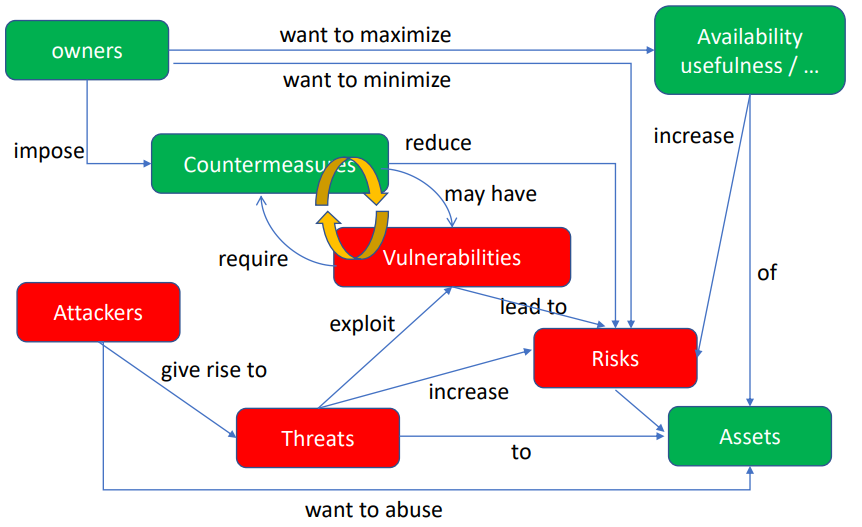
\includegraphics[scale=0.6]{chapters/02/assets/security-meta-model-def}
  \caption[Security meta-model definition. Image by prof. A. Marchetto taken from commoncriteriaportal.org.]{Security meta-model definition. Image by prof. A. Marchetto taken from \url{commoncriteriaportal.org}.}
  \label{fig:security-meta-model-def}
\end{figure}

CVE, which stands for \textit{Common Vulnerabilities and Exposures}, is a list of publicly known cybersecurity vulnerabilities. The CVE system provides a reference method for publicly known information-security vulnerabilities and exposures. Each CVE entry represents a unique identifier for a specific vulnerability, named \textit{CVE-ID}, making it easier to reference it across different tools.

Each CVE entry is evaluated using the CVSS score, which stands for \textit{Common Vulnerability Scoring System}. This system provides a standardized way to assess the severity of vulnerabilities. It is important to note that CVSS measures severity, not risk. \\
CVSS v2.0 and CVSS v3.x include three metric groups: Base, Temporal and Environmental. The Base metrics evaluate the intrinsic characteristics of a vulnerability that are constant over time and across user environments. The Temporal metrics adjust the valutation based on factors like patch availability and exploit code and the Environmental metrics allow organizations to customize the score based on their unique environment. The latest version, CVSS v4.0, introduced in 2023, includes Base, Threat, Environmental and Supplemental metric groups. Compared to the previous version, the Threat metrics evaluate the likelihood of an attacker exploiting the vulnerability, the Environmental metrics evaluate the impact of the vulnerability on the organization's unique environment and the Supplemental ones provide additional information about the vulnerability.~\cite{cvss-4-spec}\\
The metrics produce a numerical score from 0 to 10, and the assessment is also represented as a vector string, which is a concise textual representation of the values used to calculate the score.~\cite{cvss-metrics}

% TODO: Add CVEs for year or some statistics in general

NVD is the \textit{National Vulnerability Database}, a U.S. government database that contains information about known vulnerabilities, including their CVE identifiers and CVSS scores. It is maintained by NIST and serves as a comprehensive resource for organizations to evaluate security risks.

NIST (\textit{National Institute of Standards and Technology}) is a U.S. federal agency that develops cybersecurity standards, guidelines and best practices. Even if it is an American agency, its standards are widely used around the world.

\subsection{Bug}

A bug is a flaw in a system that is not behaving as it is designed to do; a vulnerability is a way of abusing the system, in a security-related way, whether that's due to a design fault or an implementation fault, so a bug.

Many security issues are related to vulnerabilities due to bugs, but not all bugs are vulnerabilities. Exploitation is an activity composed of many steps in which an attacker uses a bug to gain its goal.

\section{IT and OT Security}

IT (\textit{Information Technology}) and OT (\textit{Operational Technology}) focus on protecting different types of systems and they have distinct priorities.

IT is primarily concerned with managing electronic data, supporting business operations and facilitating decision-making through the use of computers and software to securely gather, store, process and share information; basically, it represents the internet access to the cloud we are used to interacting with every day. In contrast, OT focuses on controlling physical processes and equipment in industrial operations such as manufacturing and energy. Unlike IT, OT directly interfaces with industrial machinery and processes, addressing the physical environment and operational requirements~\cite{it-ot-diff-paloalto}, as visible in~\cref{fig:it-ot-diff}.

\begin{figure}[ht]
  \centering
  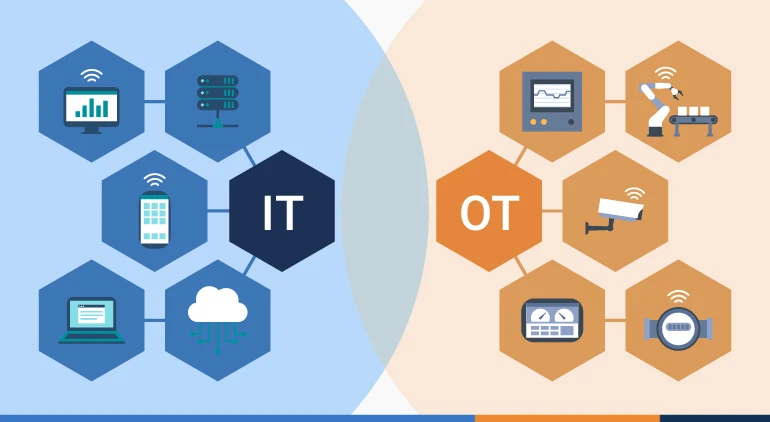
\includegraphics[width=0.9\textwidth]{chapters/02/assets/it-ot-diff.jpg}
  \caption[IT vs OT: how they differ. Image by onlogic.com]{IT vs OT: how they differ. Image by \url{onlogic.com}}
  \label{fig:it-ot-diff}
\end{figure}

We can devise some comparison points between the two types:
\begin{enumerate}
  \item \textbf{Primary priorities}: IT security prioritizes Confidentiality, Integrity and Availability (CIA), with the main focus set to protect data from breaches and authorized actions, while OT security prioritizes Availability, Integrity and Confidentiality (AIC), ensuring the continuous operation of critical systems with safety and reliability being more important than data confidentiality.
  \item \textbf{Impact of Security Breaches}: IT breaches typically affect data confidentiality and may result in privacy violations, financial losses or business disruptions. OT breaches can have severe direct consequences, including physical damage and environmental harm.
  \item \textbf{Security Measures}: IT security can use cybersecurity tools such as firewalls, antivirus, encryption and user authentication. Instead, OT security should require specialized tools like network segmentation, strict access control and real-time monitoring.
  \item \textbf{Regulatory Requirements}: The former uses regulations like GDPR, the \textit{General Data Protection Regulation} to protect personal data for a European citizen and standards like ISO-27001, while the latter follows regulations and standards like the IEC 62443, which is a series of standards for industrial automation and control systems management and security. More on these regulations in the next chapters.
  \item \textbf{Vulnerability management}: IT systems can usually be patched with a software update in a short time without severe impact on operations, while OT systems may require a longer time to be patched, as they are often critical to the operation of industrial processes or incompatible with the running legacy systems.
\end{enumerate}

Despite their distinct differences, IT vs. OT cybersecurity share similarities and are increasingly overlapping and one approach has not to exclude the other.

According to the \textit{2023 State of Operational Technology and Cybersecurity Report} by Fortinet\footnote{\url{https://www.fortinet.com}}, as shown in~\cref{fig:fortinet-intrusions-env-impacted}, nearly one-third of respondents indicated both IT and OT systems were impacted, up from the 21\% in 2022.

\begin{figure}[ht]
  \centering
  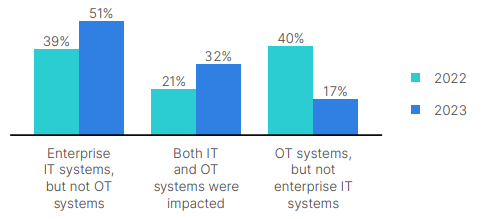
\includegraphics[scale=0.8]{chapters/02/assets/fortinet-intrusions-env-impacted.png}
  \caption[Environments impacted]{Environments impacted}
  \label{fig:fortinet-intrusions-env-impacted}
\end{figure}


As a general rule, OT devices are traditionally kept separate from the public internet and often internal networks, which means they can only be accessed by authorized employees. However, it is increasingly possible for OT systems to be controlled and monitored by IT systems or remotely via the Internet.~\cite{it-ot-cybersecurity}

\section{Industry 4.0}

Industry 4.0, synonymous of \textit{smart manufacturing}, is the realization of the digital transformation of the field, delivering real-time decision-making, enhanced productivity, flexibility and agility to revolutionize the way companies manufacture, improve and distribute their products.

This is the Fourth Industrial Revolution, characterized by increasing automation and the employment of smart machines and smart factories. By collecting more data from the factory floor and combining that with other enterprise operational data, a smart factory can achieve information transparency and better decisions.

Some specific technologies are pushing this revolution:~\cite{what-is-industry-4-0}
\begin{itemize}
  \item \textbf{Internet of Things (IoT)}: machines on the factory floor are equipped with boars that allow the machines to connect with remote services, making possible for large amounts of valuable data to be collected, analyzed and exchanged.
  \item \textbf{Cloud computing}: the typically large amount of data being stored and analyzed can be processed efficiently and cost-effectively with \textit{the cloud}. Cloud computing can also reduce startup costs for small- and medium-sized manufacturers who can right-size their needs and scale as their business grows.
  \item \textbf{AI and machine learning}: Artificial Intelligence (AI) and machine learning can create insights providing visibility, predictability and automation of operations and business processes. The data collected from these assets can help businesses perform predictive maintenance based on machine learning algorithms, resulting in more uptime and higher efficiency.
  \item \textbf{Edge computing}: to reduce latency and improve security, edge computing can be used to process the needed data closer to the source, rather than sending all the raw statistics to the cloud, wasting bandwidth and time.
  \item \textbf{Cybersecurity}: last but not least, when undergoing a digital transformation to Industry 4.0, it is essential to consider a cybersecurity approach that encompasses IT and OT equipment.
\end{itemize}

\section{Industrial devices: PLC and HMI}

Industrial devices are used in many different sectors like manufacturing, energy, transportation and so on. We can trace back these devices to a common tablet placed on a wall or on a production line, with the difference that these devices support a wide range of industrial protocols. These devices are usually not connected to the internet and they take input from a physical human interaction physically on the place.

These types of devices are an example of HMI, which stands for \textit{Human Machine Interface}, and they are defined as a feature or component of a certain entity that enables humans to engage and interact with machines. In the past HMIs started to be command line interfaces handled by a keyboard, then they evolved to graphical user interfaces with the support for the mouse navigation and now they are touchscreens, where the end-user directly touches the screen.\\
Traditionally, to integrate a manufacturing line with an HMI, the HMI had to be connected to a \textit{Programming Logic Controller} (PLC) to display the data received from the PLC and give the PLC input from users.~\cite{what-is-hmi}

In terms of the demands of Industry 4.0, industrial HMIs will also see further incorporation of new and emerging technologies that are impacting HMIs as a whole. First of all, there is the need to start integrating the Internet of Things (IoT) into industrial HMIs. This will allow for the collection of data from the factory floor and the ability to analyze that data in real-time. This will also allow for the ability to control the factory floor from a remote location. Of course, making these devices connected to the internet makes the risks of cyberattacks higher.

\section{ICS and IACS}

ICS and IACS refer respectively to \textit{Industrial Control System} and \textit{Industrial Automation and Control Systems}. In our context, they can be used interchangeably to define the collection of hardware, software and policies that control and manage the industrial process. Basically, it means that anything interacting with the system influencing its safety, security and operations belongs to IACS.~\cite{ics-or-iacs}

We use this terminology in the next chapters, especially related to the security regulations of the systems.

\section{Standards and Regulations}
Until the so-called third industrial age, or Industry 3.0, cybersecurity had minimal impact on manufacturing. Industrial machinery wasn't necessarily connected to the internet or each other, making external risks unlikely. However, with the dawn of Industry 4.0, smart machinery and smart factories have become vital for the smooth operation of production departments, placing cybersecurity at the forefront of concern.

Cybersecurity involves protecting systems, networks and programs from digital attacks. Given the critical nature of the topic and the attention it demands, companies are embarking on paths to elevate their awareness of cyberattacks, adopting internal policies, or even pursuing specific certifications in cybersecurity. Concurrently, national and international legislators have introduced new legislative measures imposing new obligations on certain entities concerning cybersecurity.

Let's now consider the most recent legislative measures on cybersecurity and the related certifications that manufacturing industries must take into account.\\
Certifications provide a guarantee of product and company security. The main certifications currently considered include:
\begin{itemize}
  \item \textbf{IEC 62443}: This series of international standards is renowned for enhancing the security of industrial control systems, setting forth fundamental prerequisites to shield industrial systems from cyber threats;
  \item \textbf{ISO/IEC 27001 (2022)}: This certification covers various aspects, including security policy, human resource security, physical and environmental security, communications management and regulatory compliance;
\end{itemize}

There are then several laws and regulations that address under various profiles the issue of cybersecurity among them it is worth noting:~\cite{cybersecurity-standards-regulations-compliance}
\begin{itemize}
  \item \textbf{Cyber Resilience Act (CRA)}~\footnote{\url{https://eur-lex.europa.eu/legal-content/EN/TXT/?uri=celex:52022PC0454}}: While still pending final approval by the European Institutions, the Cyber Resilience Act seeks to enhance the resilience of the European digital market by ensuring that connected devices and digital services are equipped to withstand cyberattacks effectively. It will become effective in 2027;
  \item  \textbf{NIS Directive 2}~\footnote{\url{https://eur-lex.europa.eu/legal-content/EN/TXT/?uri=CELEX:32022L2555}}: This directive outlines essential criteria that companies must adhere to in order to maintain a robust level of cybersecurity. These criteria cover the implementation of risk analysis strategies, fortification of information system security and effective incident management protocols. EU Member States must transpose this directive, with enforcement specified in the respective national acts;
  \item \textbf{Italian Cybersecurity Law (June 28th, 2024 No. 90)}~\footnote{\url{https://www.gazzettaufficiale.it/eli/id/2024/07/02/24G00108/sg}}: This Italian law pertains to national cybersecurity and applies to both public and private entities whose services are deemed critical. It mandates the implementation of security measures to protect critical digital infrastructures and sensitive information, including specific obligations to notify the Cybersecurity Agency of any cyber incidents;
  \item \textbf{New Machinery Regulation No. 1230/2023}~\footnote{\url{https://eur-lex.europa.eu/legal-content/EN/TXT/?uri=CELEX:32023R1230}}: This regulation will replace the Machinery Directive No. 2006/42/EC, focusing on the overall safety of machinery and semi-machinery and it will become effective in 2027. It emphasizes the essential integration of cybersecurity into the design and manufacturing processes of machinery, recognizing the potential risks that cyber vulnerabilities pose to physical safety;
\end{itemize}

\section{Security vulnerabilities scan}

A security vulnerabilities scan is a process that looks for vulnerabilities in a system or network. It is a way to identify potential security risks and weaknesses that could be exploited by attackers. The scans can be performed manually or automatically using specialized tools. The goal of this type of scan is to identify vulnerabilities and provide recommendations for improving the security of the system.

There are also different types of security scans, including network scans and penetration tests. Network scans are used to identify devices on a network and detect open ports and services while penetration tests are used to simulate cyberattacks and test the security of a system.

Security scans are an important part of a comprehensive security program. They can help organizations identify and address security vulnerabilities before they are exploited by attackers. By regularly performing security scans, organizations can improve their security attitude and reduce the risk of a security breach.

\section{JSON and YAML}

JSON, acronym of \textit{JavaScript Object Notation}, is a lightweight data-interchange format that is easy for humans to read and write and easy for machines to parse and generate. It is based on a subset of the JavaScript programming language. JSON is often used to exchange data between a server and a web application. It is a text format that is language-independent and can be used with any programming language. JSON is commonly used for configuration files, API responses and data storage.

YAML, a recursive acronym of \textit{YAML Ain't Markup Language}, is a human-readable data serialization format that is usually used for configuration files. It is a superset of JSON and is designed to be more human-readable and easier to write than JSON. It is commonly used in the cloud computing industry for configuration files and infrastructure as code.

\noindent\begin{minipage}{\linewidth}
  \vspace{0.5cm}
  \begin{lstlisting}[style=json, caption={JSON example}, label={lst:json-example}]
{
  "name": "John",
  "employed": true,
  "address": {
    "city": "Verona",
    "country": "Italy"
  },
  "hobby": ["reading", "running"]
}
  \end{lstlisting}
\end{minipage}

\noindent\begin{minipage}{\linewidth}
  \vspace{0.5cm}
  \begin{lstlisting}[style=yaml, caption={YAML example}, label={lst:yaml-example}]
name: John
employed: true
address:
  city: Verona
  country: Italy
hobby:
  - reading
  - running
  \end{lstlisting}
\end{minipage}

The example in~\cref{lst:json-example} show the data represented in JSON, while~\cref{lst:yaml-example} shows the same data as YAML.

\section{REST API}

REST stands for \textit{REpresentational State Transfer}, and it is an architectural style for designing networked applications. It relies on a stateless client-server communication protocol, meaning that each request from a client to a server must contain all the information necessary to understand the request. REST is often used in web services development as a way to communicate between client and server.

A REST API is an application programming interface that uses HTTP requests to perform operations on a server. The endpoints can be called in a RESTful way, meaning that the user transfers a representation of the state of the resource to the requester or endpoint with appropriate HTTP methods to perform standard database functions like creating, reading, updating and deleting records (also known as \textit{CRUD}) within a resource.~\cite{rest-api}

\section{Deployment of the microservices}

This section explains how a software can be deployed in a cloud environment, with a focus on the microservices architecture.

\subsection{Microservice}

Microservice architecture is an architectural style that organizes an application into a set of services that can be deployed independently and are loosely coupled. This means each service is packaged as an executable unit ready for production and that the services do not have direct dependencies on each other, allowing for independent development, deployment and scaling.~\cite{microservices-what-are}

Doing so, there is no need to scale or deploy the entire application when only a part of it needs to be updated or scaled. This approach allows for faster development and deployment cycles, as well as improved fault tolerance and scalability. The concept is shown in~\cref{fig:monolith-microservices}.

\begin{figure}[ht]
  \centering
  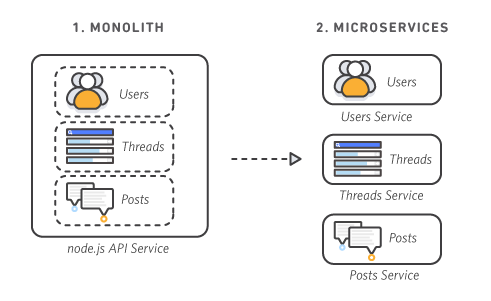
\includegraphics[scale=0.6]{chapters/02/assets/monolith-microservices.png}
  \caption[Breaking a monolithic application into microservices]{Breaking a monolithic application into microservices. Image by \texttt{aws.amazon.com}}
  \label{fig:monolith-microservices}
\end{figure}

\subsection{Virtualization}

Virtualization is a technology that enables the creation of virtual versions of physical resources such as processors, storage devices, or network components. By simulating the functions of physical hardware, virtualization allows multiple operating systems to run on a single physical machine. This approach enhances IT agility, flexibility and scalability, while also providing significant cost savings by abstracting the underlying physical hardware.~\cite{virtualization-aws}

Each virtualized environment runs within its allocated resources. There are two main types of virtualization approaches: container-based virtualization and hypervisor-based virtualization, also known as virtual machines' virtualization.

\subsubsection{Container vs. Virtual Machine}

A modern and efficient way to execute microservices is to use \textit{containers}. \\
Containers are lightweight software packages that contain all the dependencies required to execute the contained software application in a virtualized environment. They share the same kernel of the host system, but they are usually isolated from the host and from other containers and they can run different operating systems. Another advantage of containers is that they are immutable, meaning that they could be altered after their creation, but the state is restored at each execution, without considering possible further different configurations.\\
Instead, compared to the containers, \textit{virtual machines}'s goal is to virtualize the entire system hardware, therefore they are slower and heavier - resources side and disk usage side - than containers.

Since we are talking of a microservices architecture, there is the need to run multiple containers at the same time, and to manage them, from the creation to the destruction up to the recovery in case of failure or the scaling in case of high load. This is where we need an orchestration tool.

\subsection{Orchestration}

Orchestration is a term referring to the automated configuration, coordination and management of virtualization software. It is used to manage the deployment, scaling and operation of application containers. Orchestration tools are used to automate the deployment and scaling of containers, as well as to manage the networking, the storage configurations of the containers and much more. The most popular orchestration tool is Kubernetes.

\subsection{CI/CD}

A container needs an image, that is a series of instructions that defines the environment of the container, starting from the base operating system up to all the steps needed to install the final software. The image is effectively the software to be executed, and the container is its running instance. The images must be built on the source code of the software and the building process can be automated by a \textit{Continuous Integration} (CI) tool. Later, the images must be pushed to a registry, that is a repository where the images are stored, and the deployment of the images can be automated by a \textit{Continuous Deployment} (CD) tool.

CI and CD are practices that allow the developers to automate the building, testing and deployment of the software. CI is the practice of integrating the code changes of the developers into a shared repository multiple times a day, and CD is the practice of automatically deploying the code changes to the production environment. CI/CD allows the developers to detect and fix the bugs early, to reduce the risk of integration issues and to deliver the software faster and more frequently.

% terraform?

\section{Agile method}

The \textit{Agile methodology} is a project management philosophy that involves breaking the project into phases and emphasizing continuous collaboration and improvement. Teams follow a cycle of planning, executing and evaluating. Teams choose agile so they can respond to changes in the marketplace or feedback from customers quickly without derailing a year's worth of plans. The publication of the Agile Manifesto\footnote{\url{https://agilemanifesto.org}} in 2001 marks the birth of the methodology. Since then, many agile frameworks have emerged such as scrum, kanban or lean. Each embodies the core principles of frequent iteration, continuous learning and high quality in its own way.~\cite{agile-methodology}

\subsection{Scrum}

Scrum is an agile project management framework, which is different from Agile, a philosophy.\\
The definition of scrum is based on empiricism and lean thinking. Empiricism says that knowledge comes from experience and that decisions are made based on what is observed. Lean thinking reduces waste and focuses on essentials. The scrum framework is heuristic; it is based on continuous learning and adjustment to fluctuating factors by acknowledging that the team does not know everything at the start of a project and it will evolve through experience. Scrum is structured to help teams to naturally adapt to changing conditions and user requirements, with re-prioritization built into the process and short release cycles so your team can constantly learn and improve.~\cite{scrum}

Scrum artefacts help to define the product, what work has to be done to create it and who has to do it. An \textit{epic} is a large body of work that can be broken down into smaller tasks. Each of these tasks is called \textit{story} and it is a short requirement written from the perspective of an end user. The story is linked to a person in the team that has to carry it out.

The two main artefacts boards are the \textit{product backlog} and the \textit{sprint backlog}. \\
The former is a list of all the tasks that needs to be done; it is a dynamic list of features, requirements, improvements, fixes and epics, ordered by their priority. Essentially, it is a \textit{"To Do"} list.\\
The latter is a list of items selected for the current sprint cycle; the sprint cycle is a fixed period of time, usually up to four weeks. Before each sprint, the team selects items from the product backlog to work on. Epics are broken down into stories and stories are moved from the product backlog to the sprint backlog.~\cite{scrum-epic-stories}

\begin{figure}[ht]
  \centering
  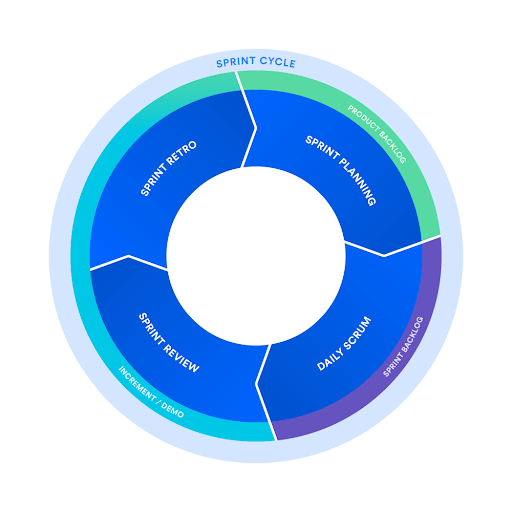
\includegraphics[width=0.8\textwidth]{chapters/02/assets/scrum}
  \caption{Scrum sprint cycle. Taken from \texttt{atlassian.com}}
  \label{fig:scrum-sprint-cycle}
\end{figure}

As visible in~\cref{fig:scrum-sprint-cycle}, Scrum is split in four principal phases:
\begin{itemize}
  \item The \textbf{sprint planning} is the initial phase of a sprint, the actual time period when the scrum team works; the team meets and decides what to do in the sprint by placing the tasks from the product backlog to the sprint backlog;
  \item The \textbf{daily scrum} is a quotidian meeting where the team members synchronize with each other. It is usually taken stand-up, as a way to not waste time and to keep the meeting short;
  \item The \textbf{sprint review} and \textbf{sprint retrospective} are the meetings at the end of the sprint where the team shows what they have done and demonstrates the work to the stakeholders and receive feedback;
\end{itemize}


      \chapter{Standards and Regulations}
\label{cha:standards}

Until the so-called third industrial age, or Industry 3.0, cybersecurity had minimal impact on manufacturing. Industrial machinery wasn't necessarily connected to the internet or each other, making external risks unlikely. However, with the dawn of Industry 4.0, smart machinery and smart factories have become vital for the smooth operation of production departments, placing cybersecurity at the forefront of concern.

Cybersecurity involves protecting systems, networks, and programs from digital attacks. Given the critical nature of the topic and the attention it demands, companies are embarking on paths to elevate their awareness of cyberattacks, adopting internal policies, or even pursuing specific certifications in cybersecurity. Concurrently, national and international legislators have introduced new legislative measures imposing new obligations on certain entities in relation to cybersecurity.

Let's now consider the most recent legislative measures on cybersecurity and the related certifications that manufacturing industries must take into account.\\
Certifications provide a guarantee of product and company security. The main certifications currently considered include:
\begin{itemize}
  \item \textbf{IEC 62443}: This series of international standards is renowned for enhancing the security of industrial control systems, setting forth fundamental prerequisites to shield industrial systems from cyber threats;
  \item \textbf{ISO/IEC 27001 (2022)}: This certification covers various aspects, including security policy, human resource security, physical and environmental security, communications management, and regulatory compliance;
\end{itemize}

There are then several laws and regulations that address under various profiles the issue of cybersecurity among them it is worth noting:~\cite{cybersecurity-standards-regulations-compliance}
\begin{itemize}
  \item \textbf{Cyber Resilient Act (CRA)}\footnote{\url{https://eur-lex.europa.eu/legal-content/EN/TXT/?uri=celex:52022PC0454}}: While still pending final approval by the European Institutions, the Cyber Resilient Act seeks to enhance the resilience of the European digital market by ensuring that connected devices and digital services are equipped to withstand cyberattacks effectively. It will become effective in 2027;
  \item  \textbf{NIS Directive 2}\footnote{\url{https://eur-lex.europa.eu/legal-content/EN/TXT/?uri=CELEX:32022L2555}}: This directive outlines essential criteria that companies must adhere to in order to maintain a robust level of cybersecurity. These criteria encompass the implementation of risk analysis strategies, fortification of information system security, and effective incident management protocols. It is imperative for EU Member States to transpose this directive by October 2024, with enforcement timelines specified in the respective national transposition acts;
  \item \textbf{Italian Cybersecurity Law (June 28th, 2024 No. 90)}\footnote{\url{https://www.gazzettaufficiale.it/eli/id/2024/07/02/24G00108/sg}}: This Italian law pertains to national cybersecurity and applies to both public and private entities whose services are deemed critical. It mandates the implementation of security measures to protect critical digital infrastructures and sensitive information, including specific obligations to notify the Cybersecurity Agency of any cyber incidents;
  \item \textbf{New Machinery Regulation No. 1230/2023}\footnote{\url{https://eur-lex.europa.eu/legal-content/EN/TXT/?uri=CELEX:32023R1230}}: This regulation will replace the Machinery Directive No. 2006/42/EC, focusing on the overall safety of machinery and semi-machinery and it will become effective in 2027. It emphasizes the essential integration of cybersecurity into the design and manufacturing processes of machinery, recognizing the potential risks that cyber vulnerabilities pose to physical safety;
\end{itemize}

This chapter will provide an overview of the most relevant standards and regulations for the context of the internship's researches, focusing on the industrial sector and the required goals; in particular, we will detail more about \textit{IEC 62443}, \textit{ISO 27001} and \textit{CRA}.

\section{IEC 62443}

The IEC 62443 provides guidelines, rules and definitions specifically crafter for any Industrial Control System (ICS) and Industrial Automation and Control Systems (IACS). Compared to ISO 27001, it is more focused on the specific sector instead of being more universal and open for the interpretation depending on the company it applies on.

The market is starting to require the IEC 62443 certification for the companies that are involved in the production of industrial devices, as it is a guarantee of the security of the product and the company itself. 

The IEC 62443 is a set of standards drafted by the \textit{Internation Electrotechnical Commission} (IEC) and it is divided into four parts:~\cite{understanding-iec-62443-parts}
\begin{enumerate}
  \item General: it covers topics that are common to the entire series;
  \item Policies and procedures: focuses on methods and processes associated with IACS security;
  \item System: it covers the requirements for the secure development and integration of systems;
  \item Component: it covers the requirements for the secure development and integration of components.
\end{enumerate}






\section{ISO/IEC 27001}








      \chapter{System}

% •	Description of the application architecture suitable for security scanning.
  % o	System Settings UI and API to control every aspect of the device
  % o	Layer diagram
% •	Design of the scanning methodology.
  % o	Aspects covered: Outdated OS, outdated libraries (e.g., OpenSSL), outdated software, default or weak credentials, insecure network communication, …
% •	Agile method, stories, backlog

% Go language
% IEC62443 findings and table
% Libraries comparison

As a reminder, the internship's company designs and builds industrial devices, as PLC or HMI. Under the hood, every PLC is powered by a custom Linux distribution, provided by ???\fcnote{ask}, that is developed by the internal \textit{Research \& Development} (R\&D) team.

In order to be able to make the device interacting with the industrial machines, the company provides a proprietary IDE software, needed to scratch projects and deploy them on the device. This software let the user define the inputs and outputs of the device, and the logic that will be executed on the device. In example, the user can define a trigger, an alarm that will be raised when a certain condition is met, a personalized handling of the data received by the many supported protocols, and so on.

Furthermore, the same IDE is used to draw the graphical interface that will be displayed on the HMI, and to define the behavior of the interface itself.\\
The graphical interface is composed by widgets, that are the building blocks of the interface. The user can define the position of the widgets, their size, their color, and their behavior. The widgets can be buttons, labels, images, graphs or custom-defined ones.

The PLC itself provides a web interface, that can be used to view and change the system settings of the device. In example, the user can change the network settings, the date and time, the management user password, the startup of the services like the SSH server, and much more. The HMI touchscreen, through dedicated gestures, let the user directly interact with the interface on-board. The web interface is powered by REST APIs, which are endpoints that can be called in a RESTful way, meaning with specific HTTP methods like GET, POST, PUT, DELETE that return a JSON response.

For the internship project we will take advantage of the REST APIs to retrieve the status of the device, and to potentially change its settings. The APIs are documented in a Swagger file, that is a JSON file that describes the endpoints, the parameters, the responses, and the authentication needed to call them. The Swagger file is used by the Swagger UI, a web interface that can be used to call the APIs and see the responses.

We can devise two different scenarios: API calls made by a remote host over a network and API calls made by the local host. In the first case, the TLS protocol secures the communication using the public-key authentication first, and then the APIs are protected by a basic authentication, that is the client must provide a management username and its related password. In the second case, the webserver listens over a "plaintext" port only accessible by the same host, and no further authentication is needed.



      \chapter{System Implementation}

This chapter describes how the system is actually being implemented.

\section{Go language interfaces}

The Go programming language provides a powerful feature called interfaces. An interface is a collection of method signatures that a type, like a struct, can implement. Interfaces allow to define a set of methods that a type must implement to be considered an instance of that interface. This allows to write code that is more flexible, especially for testing purposes.

We setup each one of the checks as a separate interface, so that we can easily test them in isolation and also to make it easier to manage the codebase and add new checks in the future, like if they are modules that can be added or removed from the system.

The modularity of a project is a key feature that allows one to easily extend the codebase and add new features. Without modularity, the codebase would be a monolithic block of code that is difficult to handle with the time and the natural growth of a codebase.

Therefore, we created different packages for the different categories of modules, like \textit{check} and \textit{version} plus some utility packages like \textit{parsing}, \textit{output} and \textit{mapping}.

The scopes for the different packages are the following:

\begin{itemize}
  \item \textit{check}: it aggregates the different controls on a property of the device, like the \textit{Check correct time} or the \textit{Check VNC credentials};
  \item \textit{version}: contains the modules to determine whether the software running on the device is up-to-date or not;
  \item \textit{parsing}: it handles the parsing of the input parameters, for example the verbose flag or the list of checks to run;
  \item \textit{output}: it manages the output of the checks, like the output format and the output file;
  \item \textit{mapping}: contains the effective available mapping for the tool.
  \item \textit{variab} and \textit{utils}: are utility packages that contain some common structures and functions that are used across the codebase.
\end{itemize}

The structure of a module is composed of the actual interface, named as \textit{<module>Interface}, where \textit{<module>} is the name of the module, a struct that implements the interface, named as \textit{<module>Struct} and a function that returns an instance of the struct, named as \textit{new<Module>}.
All the fields of the struct are private, and the public method is the one that returns the method of the interface.

A practical example is the \textit{CheckTime} module, which checks if the time of the device is correct. The interface is defined as follows:

\begin{lstlisting}[style=golang]
type checkTimeInterface interface {
	checkTime(context.Context) variab.Result
	getNtpHmiConfig(context.Context) (*hmiDateTimeDto, error)
	getRealTimeWrapper() (*time.Time, error)
}
\end{lstlisting}

The structure is defined as follows:

\begin{lstlisting}[style=golang]
type checkTimeStruct struct {
	delta             time.Duration
	getCliTime        func() (*string, error)
	getRealTime       func(string, string, string, time.Duration) (*time.Time, error)
	[omitted]
	timeout           time.Duration
}
\end{lstlisting}

There is an instance of the struct that is returned by the function \textit{newCheckTime}:

\begin{lstlisting}[style=golang]
func newCheckTime() checkTimeInterface {
	return &checkTimeStruct{
		delta:          DELTA_DURATION,
		getCliTime:     getCliTime,
		getRealTime:    getRealTime,
		[omitted]
		timeout:        utils.TIMEOUT,
	}
}
\end{lstlisting}

and the public method is the one that returns the method of the interface:

\begin{lstlisting}[style=golang]
var checkTime checkTimeInterface = newCheckTime()

func CheckTime(ctx context.Context) variab.Result {
	return checkTime.checkTime(ctx)
}
\end{lstlisting}

% Some of the variables are omitted for brevity. The other ones come from both some constants and some utility variables defined across the codebase. 
The interface has a method that checks if the time of the device is correct, and it always returns a \textit{variab.Result} struct that contains the result of the check.

The \textit{Result} structure of the package \textit{variab} is a common structure that is used to return the result of the checks. It contains a concise message for the output, an optional recommendation to solve the issue, a severity level ranging from \textit{none} to \textit{high} and an operation status, where \textit{OK} means that the module completed the task without noticing any vulnerability, \textit{ISSUE} means that the module contains a potential weakness, \textit{EXECUTION\_ERROR} in the case of an unhandled exception, \textit{UNKNOWN} otherwise. This structure is used by all the modules to return the result of a module. Any exception is handled in order to guarantee the robustness of the tool in case of any failure, allowing the user to always obtain a valid output.

\begin{lstlisting}[style=json, caption={Result struct}]
{
  "message": string,
  "recommendation": string,
  "severity": none|low|moderate|high,
  "status": OK|ISSUE|EXECUTION_ERROR|UNKNOWN
}
\end{lstlisting}

This composition is common to all the modules, and it allows us to easily test the modules in isolation, by mocking the dependencies of the struct. This is done by creating a new struct that implements the same interface, but with mocked methods, and then injecting this struct in the test. This way, we can test the module without having to actually run the code that is being mocked. This is a powerful feature of the Go language that allows to write more robust and maintainable code. More to follow about the testing phase in the next chapter.

\section{First sprint}

The first sprint has the goal of implementing the first set of modules, as expressed in the sprint planning. We are going to detail the implementation of every story from the sprint backlog.

\subsection{CheckTime module}

The \textit{CheckTime} module checks if the datetime of the device is correct. This is a fundamental thing to verify because the issues with the devices not connecting to the internet and to the cloud are most of the time due to the incorrect datetime, leading to an error with the SSL certificate. In fact, if the date is not correct, the SSL certificate could result as expired or not yet valid, warning the user that the connection is not secure.

It does so by getting the time from the device and the real-time from a remote server, and then comparing the two times. If the difference between the two times is greater than a certain threshold, expressed in a range of few minutes, then the module returns an \textit{ISSUE} status, otherwise it returns an \textit{OK} status. Of course, this module works with an active internet connection only; if the device is not connected to the internet, then the module returns a valid execution error.

To perform the execution, it runs the following steps:
\begin{itemize}
  \item first, it gets the UNIX timestamp, an integer number representing the elapsed seconds since 1\textsuperscript{st} January 1970, by executing the command \texttt{date +\%s} on the local shell;
  \item then it calls a remote endpoint that returns the real datetime;
  \item it parses the two datetimes;
  \item finally, it compares their difference and returns the result.
\end{itemize}

If any of the steps fails, the module returns the execution error status.

% proxy network call qui?

\subsection{JSON output}
\label{sec:json-output}

Every module returns a structure representing the result of the execution, a brief message and a recommendation to solve the potential issue. The modules runner collects all the results from the modules in a \textit{Report} type variable, that is defined as a map of maps, in order to have the direct mapping of the result of the module under the category and the name of the module.

The resulting type is therefore given to the \textit{output} package, which is responsible for the desired destination format. The default formatter is JSON, but it can be easily extended to support other formats like YAML by importing or implementing the corresponding marshaler, that is a function that transforms the encoding of an \textit{any} value to the desired format.

By default, the output is printed to the standard output of the terminal, but the destination can be redirected to a file by using the built-in method with the \texttt{-d} flag.

The output can be printed in a pretty format by using the \texttt{--pretty} flag, useful for human readability. Anyway, the predefined formatting is minified. The formatter can be chosen by using the \texttt{-o} flag, followed by the desired format. For example, to output the result in YAML format in the terminal the command is \texttt{./scantool scan -o yaml}, or \texttt{./scantool scan -o yaml -d output.yaml} to redirect the output to a file.

The list of the active modules is available with the command \texttt{./scantool list}, printed in the standard output of the terminal, one for line.

For example, given the execution of the datetime module only, issued with the command \texttt{./scantool scan --list "check.time" --pretty} with no further parameters, the output structure would be as the following:

\begin{lstlisting}[style=json, caption={Output of the datetime module}]
{
"check": {
  "time": {
    "message": "The current datetime is synced",
    "recommendation": "No action required",
    "severity": "none",
    "status": "OK"
  }
}
\end{lstlisting}

\subsection{Cross build script}

The Go programming language provides a powerful feature called cross-compilation. This allows to build the binary for a different architecture than the one of the machine that is building it. This is useful to build the binary for a different architecture, like ARM, that is the architecture of some of the devices that we are going to use for debugging purposes.

Go provides the built-in command \texttt{go build <file>} that builds the binary for the current architecture, but it also provides the \texttt{GOOS} and \texttt{GOARCH} environment variables that can be set to the desired values to build the binary for a different architecture.

The former is the operating system, and the latter is the architecture. Possible values useful for the project are \texttt{linux} for the operating system and \textit{arm}, \textit{arm64} and \textit{amd64} for the architecture. All the available values can be found in the official documentation of the Go programming language.~\cite{go-valid-goos-goarch-combinations}

By default, the binary includes debug symbols, that are useful for debugging purposes, but they are not necessary for the production environment. They increase the size of the binary to several megabytes, and they are not needed by the end user. In particular, we add two flags to the build command:~\cite{go-ldflags-all,go-ldflags-s-w}
\begin{itemize}
  \item \texttt{-s} turns off generation of the Go symbol table;
  \item \texttt{-w} turns off debugging information, not being able to trace the resulting binary with the \texttt{gdb} debugger.
\end{itemize}

In the context of the automatic pipeline that builds the binary for the different architectures, we also inject the version number of the binary in the build command, by using the \texttt{-X importpath.name=value} flag. This flag allows to set the value of the string variable in \textit{importpath} named \textit{name} to \textit{value}.~\cite{go-ldflags-all}

Furthermore, we also explicitly set the environment variable \texttt{CGO\_ENABLED=0} to disable the use of the machine C compiler. Anyway, that is disabled by default when cross-compiling and the go builder chooses the appropriate compiler for the target architecture.~\cite{go-cgo-compiler}

Finally, we set the \texttt{-trimpath} flag to remove the absolute path of the source files from the binary, in order to make the binary reproducible. This is a good practice to follow, as it does not leak any information about the source code and the environment where the binary was built.~\cite{go-trimpath-arg}

The resulting binary for each architecture is placed in a tree of directory, where the root directory is the version of the binary, and the subdirectories are the architectures. The filename of the binary is the same as the name of the project, that is \texttt{scantool}.

The final build command is the following:
\begin{lstlisting}[caption={Go tool cross-build command}]
  env GOOS=$GOOS GOARCH=$GOARCH CGO_ENABLED=0 go build -trimpath -ldflags="-s -w -X 'main.VERSION=$version'" -o $output_base_dir/$version/$arch/$filename main.go
\end{lstlisting}

The difference between the size of a build without any optimization and an optimized build is quite relevant. Taking as example the architecture \textit{arm64} on the \textit{Linux} operating system, the former takes 12MB and the latter takes 7.7MB. On industrial devices, such size difference matters a lot in terms of storage and bandwidth to download it on the fly when needed.

\subsection{Scan OS version}

The custom board of the industrial devices powers a custom Linux distribution, that is based on the Yocto Project. The updates are managed by the internal department of the company, with an internal version manager. The updates are not automatic, and they have to be requested by the customer.

This module monitors whether the operating system is at its latest version or not. Given that the estimated work to implement it as a single block is not trivial, we can split it into two different specializations: the first one is the one that checks the version of the operating system by retrieving the build date, and the second one is the one that checks the version of the operating system by reading the online repository.

The Device Settings API, a set of endpoints used to retrieve the information about the status of the device and to potentially change them, provides among other things the version number and the build date of the operating system. There is the \texttt{/api/v1/management/mainos} endpoint that returns a JSON object structured as follows:

\begin{lstlisting}
{
  "version": "4.2.323",
  "date": "2024-04-17T06:00:00.000Z"
}
\end{lstlisting}

The module is implemented by the \textit{versionOsInterface} and \textit{versionOsStruct} structure. The interface is defined as:

\begin{lstlisting}[style=golang]
type versionOsInterface interface {
  getOsInfo(context.Context) (*versionOsApiDto, error)
  checkOsVersion(context.Context) variab.Result
}
\end{lstlisting}

and the structure is formed of the following fields:

\begin{lstlisting}[style=golang]
type versionOsStruct struct {
  xMonthAgo      int
  [omitted]
}
\end{lstlisting}

The \textit{xMonthAgo} field is the threshold expressed in a range of few months. The \textit{getOsInfo} method retrieves the information about the operating system from the Device Settings API, and the \textit{checkOsVersion} method actually performs the comparison.

\subsubsection{Offline date based}

The first specialization of the module checks the version of the operating system by reading the build date of the system. This is done by retrieving the build date of the system from the Device Settings API, that is the \textit{date} field of the API response. The date is then compared with the current date, and if the difference is greater than a certain threshold then the module returns an issue, otherwise it returns an OK status throug the \textit{Result} structure.

\subsubsection{Online version based}

This specialization should compare the local version of the operating system with the latest version available somewhere online. Since the company does not provide a public repository for the updates, this module cannot be implemented yet. The idea is to have a list of the latest versions for the different device models and to compare the local version with the latest one. If the local version is not updated, then the module returns an issue, otherwise it returns an OK status. This is a future work that can be implemented when the company will start to provide a public repository for the updates. As a matter of fact, this story has been suspended in the context of our project.

\subsection{Default BSP credentials}

Setting common passwords is a bad practice, as they let an attacker to potentially gain unauthorized access to the management of the device.

The devices ship with some default credentials for the two users that are available on the system, named \textit{admin} and \textit{user}. The credentials are required to interact with the Device Settings.
% They are asked to be changed at the first login, but the user could skip the step and keep the default ones.\footnote{verify}

The module checks whether the default credentials are still in use by trying to login with a pre-defined set of passwords for the two users. The module performs $2*|harcodedPasswords|$ HEAD requests to an arbitrary endpoint of the Device Settings API and it checks the status code of the response. If one of the responses' status codes is \textit{200 Success}, meaning that the authorization has been granted and therefore username and password match, then the module returns an issue with a high severity, otherwise it returns an OK status.

This security control is possible without stumbling into the device's built-in authentication rate-limiting because the total number of requests is below the threshold of the requests for minute that the device accepts before temporarily blocking the access from that access.

The module is implemented by the \textit{checkCredentialsSystemSettingsInterface} and \textit{checkCredentialsSystemSettingsStruct} structure. The interface is defined as:

\begin{lstlisting}[style=golang]
type checkCredentialsSystemSettingsInterface interface {
	checkCredentialsSystemSettings(context.Context) variab.Result
}
\end{lstlisting}

and the structure is made of the following fields:

\begin{lstlisting}[style=golang]
type checkCredentialsSystemSettingsStruct struct {
  [omitted]
  hmiHeadRequest func(string, time.Duration, *string, *string) (*http.Response,error)
  users          []string
  passwords      []string
}
\end{lstlisting}

The \textit{hmiHeadRequest} function is a utility function that performs a HEAD request to the given URL with a certain user and password. The \textit{users} and \textit{passwords} fields are the list of users and passwords to try to login with.

\subsection{Scan SSH port}

The SSH protocol, which stands for \textit{Secure Shell}, is a cryptographic network protocol that allows to securely connect to a remote device. It is widely used in the industry to connect to the devices for the purposes of debugging, maintenance and monitoring. The SSH protocol is based on the client-server model, where the client connects to the server and authenticates itself by providing a username and a password or a public key. The server then verifies the credentials and grants access to the client if they are correct.

The SSH protocol is based on the TCP protocol, and it uses port 22 by default. The server, that is the industrial device, listens on port 22 for incoming connections. Because of the widespread adoption of the SSH protocol, that port is a common target for attackers who try to gain unauthorized access to the devices.

This story is a specialization of a wider set of stories that check the status of the different services running on the device. The idea is to check whether the status of the service reported by the Device Settings API matches with the actual status of the service, and if enabled to warn that a port is exposed and therefore to be informed about the potential risks.

The module is implemented by the \textit{checkServicesInterface} and \textit{checkServicesStruct} structure. The interface is defined as:

\begin{lstlisting}[style=golang]
type checkServicesInterface interface {
  checkServices(context.Context, string) variab.Result
  hmiConfig() (*hmiServicesDto, error)
}
\end{lstlisting}

and the structure is composed of the following fields:

\begin{lstlisting}[style=golang]
type checkServicesStruct struct {
  isPortOpen     func(uint, time.Duration) (bool, error)
  [omitted]
}
\end{lstlisting}

The \textit{hmiConfig} function retrieves the information about the services from the Device Settings API, and the \textit{checkServices} function actually performs the check. The API endpoint is located at \texttt{/api/v1/services} and it returns a JSON object structured as a list of objects for each service, where each object contains its id, the name and the status.

The \textit{isPortOpen} function is a utility function that checks if the port is open on the device. It works by trying to open a socket on the port defined by a predefined map that contains a list of default ports for each of the services. Depending on the protocol, the function tries to connect to each of the ports and returns true if the connection is successful, otherwise it returns false.

By combining the two functions, the module checks if the SSH port status reported by the Device Settings API matches the actual status of the port.

\subsection{Check VNC credentials}

As part of the services that are running on the device, one of them is the VNC service. VNC, which stands for \textit{Virtual Network Computing}, is a cross-platform graphical desktop sharing system to remotely control another computer. It transmits the screen of the remote device to the client, and it allows to interact with it by sending the mouse and keyboard events. It uses the RFB - \textit{Remote Framebuffer} - protocol that governs the format of the data that passes between the client and server within the VNC system. The protocol itself does not require a mandatory authentication method, but is supports many of them, like a password or a certificate.

If the service is not properly configured and does not require a password to connect, then an attacker could potentially gain unauthorized direct access to the graphical interface and perform any operation that a legitimate user could do.

The module checks whether the VNC service is configured with a password or not. It does so by retrieving the configuration, in particular the port on which the service is running, from the Device Settings API, and then implementing the protocol itself to get the required authentication method. If the authentication method is not set, then the module returns an issue with a high severity, otherwise it returns an OK status.

\subsubsection{RFB protocol}

The RFB protocol is defined in the RFC 6143~\cite{rfc6143}. It works using the TCP protocol for the transport layer. The server, that is the industrial device, listens on the default port 5900 or on a custom one defined by the customer in the Device Settings.

The protocol expects the following steps:

\begin{enumerate}
  \item the client connect to the server and the server sends the protocol version; the \textit{ProtocolVersion} message consists of 12 bytes interpreted as a string of ASCII characters in the format \texttt{RFB xxx.yyy\textbackslash n} where \texttt{xxx} and \texttt{yyy} are the major and minor version numbers, left-padded with zeros: the only published protocol versions at this time are 3.3, 3.7, and 3.8. Other version numbers are reported by some servers and clients, but should be interpreted as 3.3 since they do not implement the different handshake in 3.7 or 3.8.
  \item the client replies to the server agreeing with its supported version, which must be less or equal to the one of the server;
        \begin{itemize}
          \item if the version is 3.3, then the server directly replies with a single integer number representing the security type;
          \item otherwise, the server replies with a list of numbers representing the security types that the server supports;
        \end{itemize}
  \item at this point, instead of proceeding with the protocol, we close the connection and we return the security type.
\end{enumerate}

If the security type is equal to the number 1, the server does not require any authentication. If the number is equal to 0, this is not expected and probably something went wrong in the implementation of the protocol. Both cases return as result a high severity issue. \\
If the security type is greater or equal to number 2, then the server correctly requires some access control. Note that we said greater than two and not strictly equal to 2 because other security types exist but are not publicly documented.

\begin{figure}[ht]
  \centering
  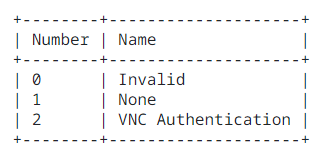
\includegraphics[width=0.5\textwidth]{chapters/05/assets/rfc6143-security-types}
  \caption{RFC 6143 security types}
  \label{fig:rfc6143-security-types}
\end{figure}

The module is implemented by the \textit{checkVncCredentialsInterface} and \textit{checkVncCredentialsStruct} structure. The interface is defined as:

\begin{lstlisting}[style=golang]
type checkCredentialsVNCInterface interface {
	checkCredentialsVNC(context.Context) variab.Result
}
\end{lstlisting}

and the structure contains the following fields:

\begin{lstlisting}[style=golang]
type checkCredentialsVNCStruct struct {
  [omitted]
  vncConn               func(string, time.Duration) (bool, net.Conn)
  vncProtocolVersion    func(net.Conn) ([]byte, error)
  vncAuthType3          func(net.Conn) (uint32, error)
  vncAuthType7_8        func(net.Conn) (uint32, error)
}
\end{lstlisting}

The \textit{vncConn} function creates the connection to the VNC server, the \textit{vncProtocolVersion} function retrieves the protocol version, the \textit{vncAuthType3} function retrieves the authentication method for version 3 of the protocol, and the \textit{vncAuthType7\_8} function retrieves the authentication method for the versions 7 and 8 of the protocol.

The \textit{checkCredentialsVNC} function performs the check by combining the functions above.

\subsection{Check certificate expiration}

The device uses the HTTPS protocol to expose the Device Settings UI and API and the optional web page of the running project. The HTTPS protocol is a secure version of the HTTP protocol that uses the SSL/TLS protocol to encrypt the data that passes between the client and the server. The SSL/TLS protocol uses a certificate to establish the identity of the server and to encrypt the data that passes between the client and the server. This behaviour is needed to prevent an attacker from intercepting the data that passes between the client and the server.

The certificate is issued by the company authority and it is valid for a certain period of time, usually years. A customer can upload a custom certificate to the device. The certificate is stored in the device.

The module checks whether the certificate is expired or not. Go provides built-in packages called \texttt{encoding/pem} and \texttt{crypto/x509} that allow to parse the certificate and to extract the expiration date. The former implements the PEM data encoding, which originated in \textit{Privacy Enhanced Mail}. The most common use of PEM encoding today is in TLS keys and certificates~\cite{go-package-pem}. The latter allows parsing and generating certificates, certificate signing requests, certificate revocation lists, and encoded public and private keys. It also provides a certificate verifier with a chain builder~\cite{go-package-x509}.

In particular, the certificate is read as bytes from the file system, then it is parsed by the \texttt{pem.Decode} function that returns a \texttt{pem.Block} structure. The \texttt{Block} structure contains the type of the block and the bytes of the block. The bytes are then passed to the \texttt{x509.ParseCertificate} function that returns a \texttt{x509.Certificate} structure. The \texttt{Certificate} structure also contains the expiration date of the certificate.

The expiration date is then compared with the current date: if the expiration date happens in less than 30 days, the module returns an issue. If the valid days left are less than 30, the severity is low; if they are less than 15, the severity is moderate; if they are less than 1, the severity is high.
-
The implementation of the module is defined by the \textit{checkCertificatesInterface} and \textit{checkCertificatesStruct} structure. The interface looks like:

\begin{lstlisting}[style=golang]
type checkCerticatesInterface interface {
	checkCertificates(context.Context) variab.Result
}
\end{lstlisting}

and the structure is made up of the following fields:

\begin{lstlisting}[style=golang]
type checkCertificatesStruct struct {
	hmiCertPath string
	loadCertFile func(string) ([]byte, error)
}
\end{lstlisting}

The \textit{hmiCertPath} field is the path to the certificate file, and the \textit{loadCertFile} function reads the certificate file from the file system. The \textit{checkCertificates} function performs the check by combining the functions above.

\subsection{Verbose flag}

This flag is a common one that is used in the command line interface of the tool to increase the verbosity of the output. By default, the output is minimal and it contains only the result of the checks, but by using the \texttt{--verbose} flag the output is increased to include more information about the execution of the modules.

The flag is implemented by taking advantage of the hooks provided by \textit{spf13/cobra}, that is the package that we use to implement the command line interface. The \texttt{cobra.Command} structure provides a \texttt{PersistentPreRun} callback that is called before the execution. We use this callback to set the verbosity level of the output for the \textit{zerolog} package with the \texttt{zerolog.SetGlobalLevel} function.

This flag is defined as persistent, meaning that it is available for every command and subcommand and it is only defined once.

\subsection{Add YAML report formatter}

In addition to the JSON output, we also add the YAML output format. The YAML format is a human-readable data serialization standard that can be used in conjunction with all programming languages and is often used to write configuration files. The YAML format is more human-readable than the JSON format. It is not native in the Go programming language, but there is an official porting available at the \texttt{gopkg.in/yaml.v3} package.

As described in~\cref{sec:json-output}, the output package is responsible for the output of the results in the desired format. The default format is JSON, but it can be easily extended to support other formats like YAML by importing the corresponding marshaler.

In this case, we add the \texttt{yaml.Marshal} function to the output package the \textit{Report} structure. If the user specifies the \texttt{-o yaml} flag, then the output is formatted in YAML to the desired destination.

The high modularity of the Go language and of the project allows to easily extend the output formats by simply adding few lines of code. This is a powerful feature of the Go language that allows to write more maintainable code.

\section{First sprint retrospective}

The first sprint has been completed successfully. All the expected modules but one have been implemented. For each of the tests, we have written comprehensive unit tests that run on demand. The implementation of the modules has been straightforward. The use of the interfaces has allowed to easily test the modules in isolation, by mocking the dependencies of the struct.

The only module that has not been implemented is the one that checks the version of the operating system by reading the online repository. This is because the company does not provide a public repository for the updates, and therefore we cannot implement the module yet. This is a future work that can be implemented when the company will provide a public repository for the updates.

Given that the first sprint has been completed successfully, we can move on to the second sprint. We did a meeting to show the results of the sprint to the office and to discuss the next steps. The feedback has been positive, and the team is happy with the results. The next sprint focuses on the implementation of more server side utilities and some more modules.

\section{Second sprint}

The second sprint has the goal of implementing the following set of modules:

\begin{itemize}
  \item Create cloud web app
  \item Implement proxy network call
  \item Automatic build and deployment
  \item Enable to download latest version of the tool
  \item Support internationalization
\end{itemize}

These are new features useful for the future adoption of the tool in the company.

The first two are server side utilities that are needed to prepare the infrastructure for future development of the tool in terms of strictly network policies and user billing. In fact, the company is interested in the possibility to offer the tool as a service to the customers, and therefore it is necessary to have a server side application in order to handle the functioning. Furthermore, as previously said, industrial network policies are very strict and usually they do not allow to connect directly to the internet, and therefore a proxy is needed to perform the network calls. \\
For example, given the case of a version check, if the remote location on which the version is stored happens on a third-party endpoint, like for an external dependency, each network administrator for each customer should manually allow the connection to that location, and beforehand the company should provide the list of the locations to allow and keep it updated. In order to avoid this, the company can provide a proxy server that is the only one that connects to the internet. The tool can then connect to the proxy server. This way, network administrators only have to allow the connection to the proxy server, that is already expected for the standard operation of the device.

The second and third points are about the automatic build and deployment of the tool. The company is interested in the possibility to automatically build the tool for the different architectures and to deploy it on the devices. This is also useful for testing purposes, as the build is preceded by the execution of the tests and also for the continuous integration and continuous deployment of the tool.

The latest point aims to provide internationalization, that is the support for different languages. The company is interested in the possibility to offer the tool in different languages, in order to make it more accessible to customers.

\subsection{Create cloud web app}

Recalling~\cref{sec:platform-applications}, the cloud app is an entire runtime made by a frontend and a backend that is visible through the platform website. The frontend is a VueJS application and the backend uses NestJS as the framework for handling the controllers, the models and the logic. Both the frontend and the backend are written in TypeScript and both implement the authentication with the platform, as it is really integrated with the platform itself and cannot be used in a standalone mode.

The skeleton of the application is generated by a public utility developed by the company, which is available on the public NPM registry. This utility generates the boilerplate code for the frontend and the backend, with many features already implemented, like the authentication with the platform, basic routing, controllers and models needed to complete the first installation on the platform.

The app also provides a running configuration of \textit{PostgreSQL} database that is used to store its data. The database is also deployed on the Kubernetes cluster.

The application has to be deployed on a Kubernetes cluster. The code also contains the required chart files, customized for the application, that are used by the Helm package manager to deploy the application on the cluster, and the Dockerfile that is used to build the Docker image of the application.

Once the deployment is live on the cluster, the application can be linked to the platform store by using the public REST API of the platform. Doing so, the application is visible on the platform website and it can be accessed by the customers.

\subsection{Implement proxy network call}

As said, usually the industrial networks attached to the devices are very strict and do not allow to communicate with every host on the internet. This is a security measure that is taken to reduce the risks of exposing relatively weak devices. In fact, according to internal statistics, unfortunately the devices are usually not updated frequently by the customers and they are not patched for the latest vulnerabilities. The goal of the tool described in this thesis is also to make aware the customers of a potential vulnerability that could be exploited by an attacker and new available updates. In order to do so, the tool has to communicate with the internet to check the latest version of the software. How to do that given all the constraints?

The solution we thought is to provide a proxy server that is the only one that connects to the final endpoints. The tool can then connect to the proxy server. This way, network administrators only have to allow the connection to the proxy server, that is already expected for the standard operation of the device.

The proxy server is managed by a controller on the cloud app backend. The controller is responsible for handling the incoming requests from the tool and for forwarding them to the respective methods. The controller is also responsible for handling the authentication with the platform. It is written in TypeScript and it uses the NestJS framework.

The proxy controller is a class that is decorated with the \texttt{@Controller} decorator, that is provided by the NestJS framework, with the parameter that is the base path of the controller. All the requests starting with that path are handled by the controller. A decorator is a special declaration that can be attached to a class, method or property, and it is used to modify their behaviour. The class is also decorated with \texttt{@ApiTags}, needed to generate the OpenAPI documentation, and by a \texttt{@UseInterceptors} directive with the \textit{LoggingInterceptor} custom one that logs the incoming requests. \\
The class contains the declaration of the services that are used by the controller to perform the actual operations. The services are injected into the constructor of the class, aka they are already instantiated when the class is defined. The class also contains the methods that are the actual endpoints of the controller. The methods are decorated with the \texttt{@Get}, \texttt{@Post}, \texttt{@Put} or \texttt{@Delete} decorators, depending on the HTTP method that they handle. The methods also contain the logic to handle the incoming requests and to return the responses. The responses are returned in the form of specific \textit{DTO}s, which stands for \textit{data transfer object} and it is an object that carries data between processes, automatically serialized by the NestJS framework to the JSON format.

The decorators starting with \texttt{@Api} are used to generate the OpenAPI documentation. The \texttt{@ApiTags} decorator is used to specify the category of the endpoint and the \texttt{@ApiHeader} decorator is used to specify the header parameters that are required. The \texttt{@ApiBearerAuth} decorator is used to specify that the endpoint requires a bearer token to be accessed. The \texttt{@UseGuards} decorator is used to specify the guards that are used to protect the endpoint from unauthorized access. In our case, we use the two custom guards \texttt{AuthGuardFromHeaders} and \texttt{InstallationRoleGuard} to respectively obtain the bearer token and the expected parameters from the headers and to confirm that the request comes from a valid app installation.

An example of the proxy controller class is shown in~\cref{lst:proxy-controller}.

\begin{lstlisting}[language=Javascript, caption={Proxy controller class}, label={lst:proxy-controller}]
[... imports ...]

@Controller('v1/proxy')
@ApiTags('Proxy')
@ApiHeader({ name: 'x-instance-id', required: true })
@ApiHeader({ name: 'x-organization-id', required: true })
@ApiHeader({ name: 'x-device-id', required: true })
@ApiBearerAuth()
@UseInterceptors(LoggingInterceptor)
@UseGuards(AuthGuardFromHeaders, InstallationRoleGuard)
export class ProxyController {
  private readonly _logger: Logger;

  private readonly _proxyTimeService: IProxyTimeService;

  constructor(
    @Inject('IProxyTimeService') proxyTimeService: IProxyTimeService,
    logger: Logger
  ) {
    this._proxyTimeService = proxyTimeService;
    this._logger = logger;
  }

  @Get('time')
  @UseGuards(RateLimiter({ max: 1 }))
  async time() {
    this._logger.info('time');

    const filteredApi = await this._proxyTimeService.ntp();

    return filteredApi;
  }
}
\end{lstlisting}

The \textit{proxyTimeService} service is the one that actually retrieve the real-time from a public NTP server. NTP stands for \textit{Network Time Protocol} and it is a protocol used to synchronize the clocks of computer systems over a network. The service is injected in the constructor of the controller, which means that there is no need to explicitly instantiate it. The service is defined by an interface that contains the methods that are needed to perform the operations. The service is then implemented by a class that implements the interface and that contains the actual logic to perform the operations. The service is responsible for handling the business logic of the application, and it is used by the controller to perform the actual operations.

An example of the proxy service class is shown in~\cref{lst:proxy-service}.

\begin{lstlisting}[language=Javascript, caption={Proxy service class}, label={lst:proxy-service}]
[... imports ...]

export class NtpTimeDto {
  time: Date;

  constructor(timestamp: Date) {
    this.time = timestamp;
  }
}

export interface IProxyTimeService {
  ntp(): Promise<NtpTimeDto>;
}

@Injectable()
export class ProxyTimeService implements IProxyTimeService {
  private readonly _logger: Logger;

  private readonly _ntpServerUrl = 'time.cloudflare.com';
  private readonly _ntpServerTimeout = 5000;

  constructor(logger: Logger) {
    this._logger = logger;
  }

  private async getNtpTime(url: string, timeout: number): Promise<NTPPacket> {
    this._logger.info(`NTP client call to url '${url}'`);
    const ntpClient: NTP = new NTP(url, 123, { timeout });
    return ntpClient.syncTime();
  }

  async ntp(): Promise<NtpTimeDto> {
    this._logger.info('ntp');

    const ntpTime = await this.getNtpTime(this._ntpServerUrl, this._ntpServerTimeout);

    return new NtpTimeDto(ntpTime.time);
  }
}
\end{lstlisting}

The interface contains the public definition for the \texttt{ntp} method, then implemented by the \texttt{ProxyTimeService} class. The \textit{NtpTimeDto} class is a data transfer object that is used to carry the data between the service and the controller.

\subsection{Automatic build and deployment}

The continuous integration and continuous deployment of the tool is a crucial part of the development process: it allows to automatically build the tool for the different architectures and deploy them to different environments. It is also useful for testing purposes, as the build is preceded by the execution of the tests.

The environments need the following set of images:
\begin{itemize}
  \item the tool written in Go language is built for three different architectures: \textit{amd64}, \textit{arm} and \textit{arm64};
  \item the frontend and the backend are built into two different sets of images, each exported for both \textit{amd64} and \textit{arm64};
\end{itemize}

About the tool, different images are needed for the devices running the \textit{arm*} architectures. \\
Instead, the frontend and the backend images are built for the cluster environment, that is the \textit{amd64} architecture on the Google Cloud Platform Kubernetes cluster, and for the development runtime where the laptops are based both on \textit{amd64} and \textit{arm64} architecture. This way, each developer can run its own instance of the cluster on its laptop and directly test the application as it would be deployed on the real cluster.

The automatic build and deployment is managed by the Google Cloud Build service. It is directly integrated with the project's repositories and it is triggered by the push of the code on a specific tag or on the master branch. The service is programmed by a configuration file, called \textit{Dockerfile}, which contains all the steps that are needed to build the images. The images are then pushed to a remote registry and then they are automatically deployed to the cluster. Instead, the built tool binaries are stored in a public storage bucket. The bucket always contains the reference to the latest master version and all the previous tagged versions. We decided to store the binaries in a public storage bucket because of the simplicity of the service for our internship project.

Therefore, the storage looks like a tree of directories, where the root directory is the version of the binary, and the subdirectories are the architectures. The filename of the final binary is the name of the tool. The tree is structured as follows:

\begin{lstlisting}[caption={Storage bucket tree of directories}]
  .
  |-- 0.1.0
  |   |-- linux-amd64
  |   |   |-- scantool
  |   |-- linux-arm
  |   |   |-- scantool
  |   |-- linux-arm64
  |       |-- scantool
  |-- 0.1.1
  |   |-- linux-amd64
  |   |   |-- scantool
  |   |-- linux-arm
  |   |   |-- scantool
  |   |-- linux-arm64
  |       |-- scantool
  |-- latest
      |-- linux-amd64
      |   |-- scantool
      |-- linux-arm
      |   |-- scantool
      |-- linux-arm64
          |-- scantool
\end{lstlisting}

Doing so, the developers can focus on the development of the tool and they do not have to worry about the building and deploying process.

\subsection{Enable to download latest version of the tool}

Recalling the tool, it is a command line software that is used to scan the device for potential misconfigurations on its settings. The tool is run on the terminal of the device, and therefore it is required to obtain the executable file. To enable the customers to download the latest version of the tool, we provide a public endpoint that returns the latest version for the different architectures.

The cloud app frontend is powered by these endpoints to assist the testers and the customers in downloading the latest version of the tool. The frontend is a VueJS application, part of the cloud app. For the internship purposes, we shipped a simple frontend composed of a dropdown that lists the available architectures, a \textit{download} button that get binary and a \textit{copy command} to copy the \textit{curl}\footnote{\url{https://curl.se/}} command, to simplify the download process by not involving the copy between the local host and the remote device. This way, the customer can easily copy and paste the command and execute it on the terminal of the device. \cref{fig:cloud-app-frontend} shows the frontend.

\begin{figure}[ht]
  \centering
  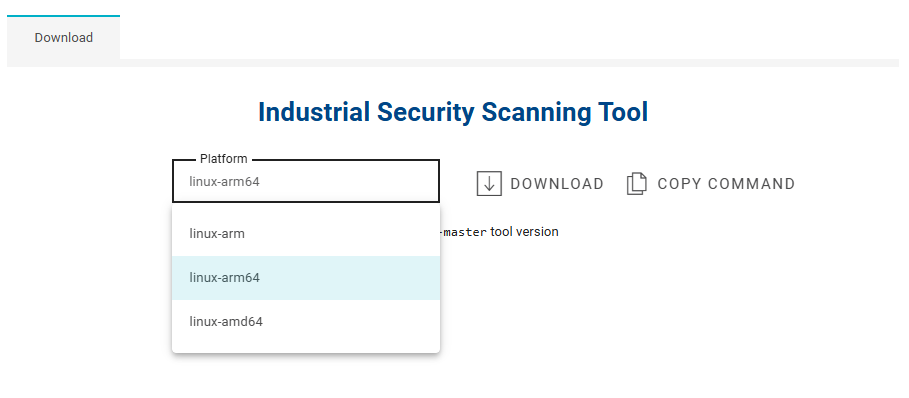
\includegraphics[width=1.0\textwidth]{chapters/05/assets/cloud-app-frontend}
  \caption{Cloud app frontend}
  \label{fig:cloud-app-frontend}
\end{figure}

The endpoint is a public REST API that is implemented by a controller on the cloud app backend. The controller is responsible for handling the incoming requests from the frontend and for forwarding them to the respective methods. The controller is also responsible for handling the authentication with the platform. The controller asks the related service model to actually list the available architectures and returns the final download link.

The endpoint is available at the \texttt{/v1/cli-release} base path; in particular, the \texttt{/platforms} path returns a dynamic list of the available architectures at that time, and the \texttt{/:version/:platform} path returns the actual download link for the specific version and platform. The download link is a direct link to the storage bucket that contains the binaries.

Notice that, although the app is accessible using a private account but the download link is public, we do not consider this a security issue because of the initial stage of the project and the limited access to the preview version of the app. In fact, only the company testers can access it at this time. Future work will be to implement a proper authentication system to access the download link.

\subsection{Support internationalization}

The support for different languages is a fundamental step for a company with a global presence. The company is interested in the possibility to offer the tool in different languages, in order to make it more accessible to customers.

In order to support internationalization, also known as \textit{i18n} because of the 18 letters between the \textit{i} and the \textit{n}, we use the \texttt{vue-i18n} package to translate the cloud app. The package is a plugin for VueJS that provides the i18n features to the application and it is available on the public NPM registry. The package allows to define the translations in a JSON file and to use them in the application by using the \texttt{\$t} function. The package also provides the ability to switch the language at runtime.

Also the tool is translated into different languages, primarily in English and Italian. The translations are again stored in different YAML files, one for each language, and they are loaded at runtime by the tool. The tool uses the \texttt{go-i18n} package. We did some wrapper functions to make the package similar to the way it works in the application by exposing a \texttt{t} function used to return the translation of a key. We decided to use a YAML translation file because it is even easier to read and write than a JSON file.

Both the translation methods support the variable replacement, that is the ability to replace a placeholder in the translation with a value. This is useful for example to translate a sentence that contains a variable part, like a number or a name. Also, they support pluralization, that is the ability to translate a sentence in different ways depending on the number of items. A clear example is the translation of the word \textit{item} in English, which is translated in two different ways depending on the number of items: \textit{item} for one item and \textit{items} for zero or more than one item. The pluralization is done by using the \texttt{one}, \texttt{other} and \texttt{few} keys in the translation file. The \texttt{one} key is used for the singular form, the \texttt{other} key is used for the plural form, and the \texttt{few} key is used for the few form. The package automatically selects the correct form based on the number of items passed as parameter.

Usually, the names of these functions are very short to reduce the verbosity in the code, given that they are used really really often in the code.

\section{Second sprint retrospective}

With this last task done, the second sprint has been completed successfully. All the expected modules have been implemented. The implementation of the modules has been straightforward. Compared to the first sprint, we adjusted the estimation of the complexity and the time needed to develop the new features and we have been able to complete the sprint in time. This is the end of the internship period. The company is satisfied by our job and it looks forward to further development.



      \chapter{Testing and Deployment}




      \chapter{Conclusions}

The increased connectivity of legacy devices, driven by the integration of the Industrial Internet of Things and digital technologies, has significantly expanded the cyberattack surface in industrial sectors.

This thesis has presented an approach to secure industrial devices by acknowledging the customers of potential risks in the configuration of their devices fleet.

The analysis of the industrial regulations and standards raised the need for a security framework that can be used to assess the security of industrial devices. Therefore, the presented scanning tool is a response to this need.

First, we have identified the main security requirements for such devices, by analyzing the most common regulations and standards. Some common requirements are shared among the regulations and others are specific to a single regulation due to the different sectors that they are focused on. The scanning tool has been designed to cover those requirements for which a solution can be taken by the customer through the configuration of the device, without the need for a hardware or software update.

The scanning tool is able to identify the misconfigurations of the industrial devices and to provide the customers with a report that can be used to improve their security, by lowering the risks. At the end of the internship period, the scanning tool was able to be run locally on a device terminal and provide the customers with a text report.

Future work should be focused on the improvement of the user experience of the tool, by providing a graphical user interface where the results are stored and can be easily accessed by the customers. That should be the expansion of the existing cloud application. Furthermore, the experience should be simplified on the device side also, to not have the customer run the tool on a terminal, but through another user interface accessible on the device along with the existing settings.

One of the requirements given by the laws is periodic scanning: although it is not been implemented in the scanning tool itself, it can be already achieved by taking advantage of a local cron job that runs it periodically, or by performing further changes to be able to remotely schedule the scanning from the cloud application.

It has been a great experience to work on this project and to be able to contribute to the security of industrial devices. I am grateful to Corvina and Exor for the opportunity to work on this project from scratch.


      \chapter{Conclusion}



      
    \endgroup


    % bibliography - bibtex format
    %
    % add chapter to index
    \addcontentsline{toc}{chapter}{Bibliography}
    % alphabetical order of authors
    \bibliographystyle{plain}
    \bibliography{biblio}
%%%%%%%%%%%%%%%%%%%%%%%%%%%%%%%%%%%%%%%%%%%%%%%%%%%%%%%%%%%%%%%%%%%%%%%%%%
%%%%%%%%%%%%%%%%%%%%%%%%%%%%%%%%%%%%%%%%%%%%%%%%%%%%%%%%%%%%%%%%%%%%%%%%%%
%% Nota
%%%%%%%%%%%%%%%%%%%%%%%%%%%%%%%%%%%%%%%%%%%%%%%%%%%%%%%%%%%%%%%%%%%%%%%%%%
%% In the bibliography, all the sources consulted for the dissertation 
%% have to be cited and listed in alphabetical order by the 
%% first author's surname.
%%
%% According to the source material, the quotation has to be as follows:
%%
%% BOOKS
%% Surname and initial/s of the name/s of the author/s, date of edition,
%% publishing house and (if applicable) number of edition.
%% 
%% JOURNAL ARTICLES 
%% Surname and initial/s of the first name/s of the author/s,
%% title of the article, name of the journal, volume number, issue number
%% and page numbers.
%% 
%% CONFERENCE PAPERS
%% Surname and initial/s of the name/s of the author/s,
%% year of the conference, title of the article, name of the conference,
%% place of the conference, conference dates, page numbers.
%% 
%% CITING WEB RESOURCES
%% The consulted webpages have to be listed in alphabetical order. 
%% It is necessary to:
%%   - Copy the specific URL (the web address) of the consulted webpage
%%   - If available, indicate the surname and first name of the author/s,
%%     the title and subtitle of the text
%%   - If available, indicate the last date you retrieved the webpage
%%     (day/month/year).   
%%%%%%%%%%%%%%%%%%%%%%%%%%%%%%%%%%%%%%%%%%%%%%%%%%%%%%%%%%%%%%%%%%%%%%%%%%
%%%%%%%%%%%%%%%%%%%%%%%%%%%%%%%%%%%%%%%%%%%%%%%%%%%%%%%%%%%%%%%%%%%%%%%%%%
    

    % \titleformat{\chapter}
        % {\normalfont\Huge\bfseries}{Appendix \thechapter}{1em}{}
    % Appendix / attachment section - optional
    % \appendix
    % \chapter{Title first appendix}

Lorem ipsum dolor sit amet, consectetur adipiscing elit. Donec sed nunc orci. Aliquam nec nisl vitae sapien pulvinar dictum quis non urna. Suspendisse at dui a erat aliquam vestibulum. Quisque ultrices pellentesque pellentesque. Pellentesque egestas quam sed blandit tempus. Sed congue nec risus posuere euismod. Maecenas ut lacus id mauris sagittis egestas a eu dui. Class aptent taciti sociosqu ad litora torquent per conubia nostra, per inceptos himenaeos. Pellentesque at ultrices tellus. Ut eu purus eget sem iaculis ultricies sed non lorem. Curabitur gravida dui eget ex vestibulum venenatis. Phasellus gravida tellus velit, non eleifend justo lobortis eget. 

\section{Title}
Lorem ipsum dolor sit amet, consectetur adipiscing elit. Donec sed nunc orci. Aliquam nec nisl vitae sapien pulvinar dictum quis non urna. Suspendisse at dui a erat aliquam vestibulum. Quisque ultrices pellentesque pellentesque. Pellentesque egestas quam sed blandit tempus. Sed congue nec risus posuere euismod. Maecenas ut lacus id mauris sagittis egestas a eu dui. Class aptent taciti sociosqu ad litora torquent per conubia nostra, per inceptos himenaeos. Pellentesque at ultrices tellus. Ut eu purus eget sem iaculis ultricies sed non lorem. Curabitur gravida dui eget ex vestibulum venenatis. Phasellus gravida tellus velit, non eleifend justo lobortis eget. 

\subsection{Sub-title}
Lorem ipsum dolor sit amet, consectetur adipiscing elit. Donec sed nunc orci. Aliquam nec nisl vitae sapien pulvinar dictum quis non urna. Suspendisse at dui a erat aliquam vestibulum. Quisque ultrices pellentesque pellentesque. Pellentesque egestas quam sed blandit tempus. Sed congue nec risus posuere euismod. Maecenas ut lacus id mauris sagittis egestas a eu dui. Class aptent taciti sociosqu ad litora torquent per conubia nostra, per inceptos himenaeos. Pellentesque at ultrices tellus. Ut eu purus eget sem iaculis ultricies sed non lorem. Curabitur gravida dui eget ex vestibulum venenatis. Phasellus gravida tellus velit, non eleifend justo lobortis eget. 


\chapter{Title first appendix}

Lorem ipsum dolor sit amet, consectetur adipiscing elit. Donec sed nunc orci. Aliquam nec nisl vitae sapien pulvinar dictum quis non urna. Suspendisse at dui a erat aliquam vestibulum. Quisque ultrices pellentesque pellentesque. Pellentesque egestas quam sed blandit tempus. Sed congue nec risus posuere euismod. Maecenas ut lacus id mauris sagittis egestas a eu dui. Class aptent taciti sociosqu ad litora torquent per conubia nostra, per inceptos himenaeos. Pellentesque at ultrices tellus. Ut eu purus eget sem iaculis ultricies sed non lorem. Curabitur gravida dui eget ex vestibulum venenatis. Phasellus gravida tellus velit, non eleifend justo lobortis eget. 

\section{Title}
Lorem ipsum dolor sit amet, consectetur adipiscing elit. Donec sed nunc orci. Aliquam nec nisl vitae sapien pulvinar dictum quis non urna. Suspendisse at dui a erat aliquam vestibulum. Quisque ultrices pellentesque pellentesque. Pellentesque egestas quam sed blandit tempus. Sed congue nec risus posuere euismod. Maecenas ut lacus id mauris sagittis egestas a eu dui. Class aptent taciti sociosqu ad litora torquent per conubia nostra, per inceptos himenaeos. Pellentesque at ultrices tellus. Ut eu purus eget sem iaculis ultricies sed non lorem. Curabitur gravida dui eget ex vestibulum venenatis. Phasellus gravida tellus velit, non eleifend justo lobortis eget. 

\subsection{Sub-title}
Lorem ipsum dolor sit amet, consectetur adipiscing elit. Donec sed nunc orci. Aliquam nec nisl vitae sapien pulvinar dictum quis non urna. Suspendisse at dui a erat aliquam vestibulum. Quisque ultrices pellentesque pellentesque. Pellentesque egestas quam sed blandit tempus. Sed congue nec risus posuere euismod. Maecenas ut lacus id mauris sagittis egestas a eu dui. Class aptent taciti sociosqu ad litora torquent per conubia nostra, per inceptos himenaeos. Pellentesque at ultrices tellus. Ut eu purus eget sem iaculis ultricies sed non lorem. Curabitur gravida dui eget ex vestibulum venenatis. Phasellus gravida tellus velit, non eleifend justo lobortis eget. 




\end{document}
